\begin{flushright} {\tiny {\color{gray} basis\_p1p\_2D.tex}} \end{flushright}
%~~~~~~~~~~~~~~~~~~~~~~~~~~~~~~~~~~~~~~~~~~~~~~~~~~~~~~~~~~~~~~~~~~~~~~~~~~~~~~~~~~~~~~~~~~~~~~~~~~

As we will see in Section~\ref{pair:mini} the above $P_1$ can be enriched 
with a so-called bubble function.
The \index{general}{Bubble Function} bubble function of the MINI element 
is described in Arnold \etal (1984) \cite{arbf84} as being $\lambda_1\lambda_2\lambda_3$
where $\lambda_i$ are the so-called barycentric 
coordinates\footnote{\url{https://en.wikipedia.org/wiki/Barycentric\_coordinate\_system }}.
\index{general}{Barycentric Coordinates}

\begin{eqnarray}
\lambda_1 &=& \frac{(y_2-y_3)(x-x_3)+(x_3-x_2)(y-y_3)}{(y_2-y_3)(x_1-x_3)+(x_3-x_2)(y_1-y_3)} \nn\\
\lambda_2 &=& \frac{(y_3-y_1)(x-x_3)+(x_1-x_3)(y-y_3)}{(y_2-y_3)(x_1-x_3)+(x_3-x_2)(y_1-y_3)} \nn\\
\lambda_3 &=& 1-\lambda_1-\lambda_2 \nn
\end{eqnarray}

\begin{center}
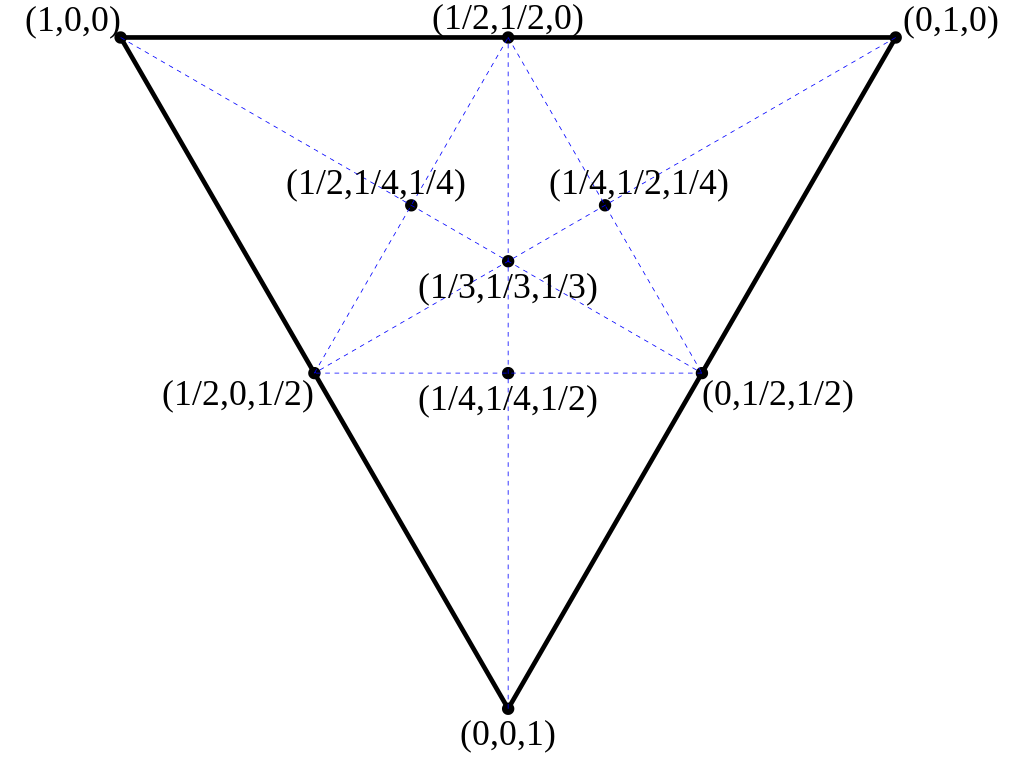
\includegraphics[width=5cm]{images/mini/barycoord1}
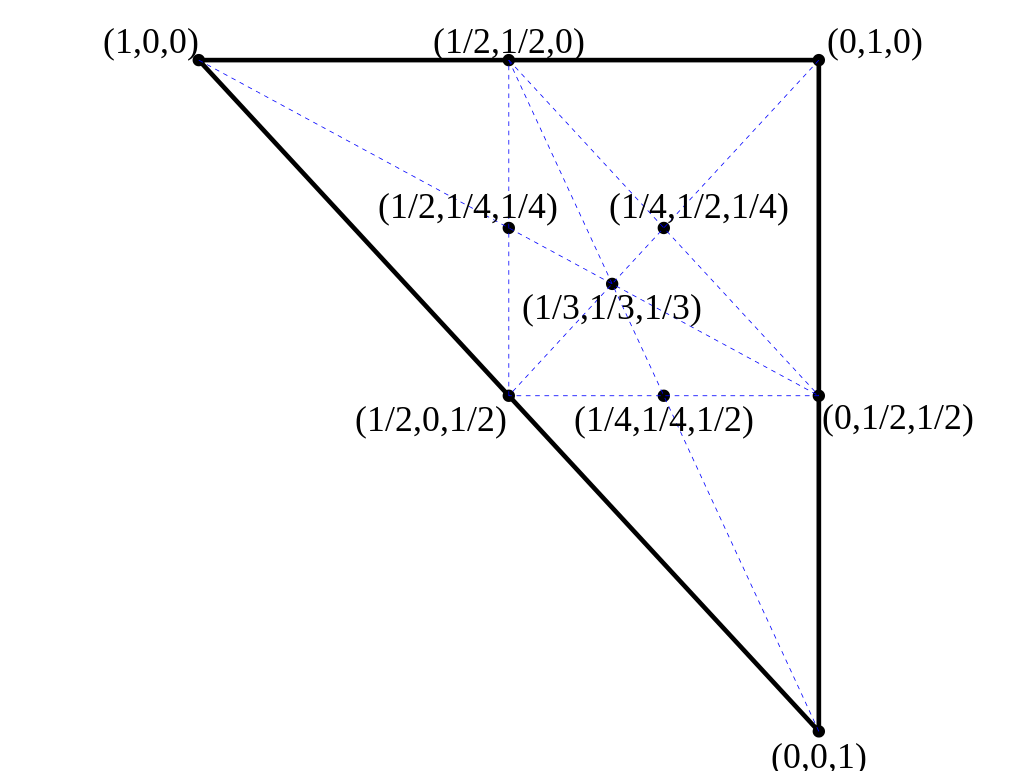
\includegraphics[width=5cm]{images/mini/barycoord2}\\
{\captionfont Barycentric coordinates ($\lambda _{1},\lambda _{2},\lambda _{3}$) on an equilateral triangle and on a right triangle.}
\end{center}

In the reference triangle, the barycentric coordinates write
\begin{eqnarray}
\lambda_1 &=& \frac{(s_2-s_3)(r-r_3)+(r_3-r_2)(s-s_3)}{(s_2-s_3)(r_1-r_3)+(r_3-r_2)(s_1-s_3)} = \frac{(-1)(r)+(-1)(s-1)}{(-1)(0)+(-1)(-1)} = -r-s+1  \nn\\
\lambda_2 &=& \frac{(s3-s1)(r-r3)+(r1-r3)(s-s3)}{(s2-s3)(r1-r3)+(r3-r2)(s1-s3)} = \frac{(1)(r)+(0)(s-1)}{(-1)(0)+(-1)(-1)} = r \nn\\
\lambda_3 &=& 1-\lambda_1-\lambda_2 = 1 - (-r-s+1) - r = s \nn
\end{eqnarray}
As we have seen before the bubble function is given by $\lambda_1\lambda_2\lambda_3 = (1-r-s)rs$
and the polynomial form for the basis functions is given by:
\[
f(r,s) =a+br+cs + d (1-r-s)rs
\]
Setting the location of the bubble at $r=s=1/3$, i.e. $\lambda_1\lambda_2\lambda_3 = 1/3$, 
we then have 
\begin{eqnarray}
f(r_1,s_1)&=&f_1 = a+br_1+cs_1 + d (1-r_1-s_1)r_1s_1 = a \nn\\
f(r_2,s_2)&=&f_2 = a+br_2+cs_2 + d (1-r_2-s_2)r_2s_2 = a + b \nn\\
f(r_3,s_3)&=&f_3 = a+br_3+cs_3 + d (1-r_3-s_3)r_3s_3 = a + c \nn\\
f(r_4,s_4)&=&f_4 = a+br_4+cs_4 + d (1-r_4-s_4)r_4s_4 = a + \frac{b}{3} + \frac{c}{3} + \frac{1}{27} \nn
\end{eqnarray}
where point 4 is the location of the bubble.
This yields
\[
a=f_1 
\quad\quad\qquad
b=f_2-a = f_2-f_1
\quad\quad\qquad
c=f_3-a = f_3-f_1
\]
and
\[
d=27\left(f_4-a-\frac{b}{3} - \frac{c}{3}\right) = 27 \left(f_4 - f_1 - \frac{f_2-f_1}{3} - \frac{f_3-f_1}{3} \right)
=27 \left(f_4 - \frac{f_1}{3}  - \frac{f_2}{3}  - \frac{f_3}{3} \right)
\] 
Finally
\begin{eqnarray}
f(r,s) 
&=&a+br+cs + d (1-r-s)rs \nn\\
&=& f_1 + (f_2-f_1)r + (f_3-f_1)s + 27 \left(f_4 - \frac{f_1}{3}  - \frac{f_2}{3}  - \frac{f_3}{3} \right) (1-r-s)rs \nn\\
&=& [1-r-s-9(1-r-s)rs] f_1 + [r-9(1-r-s)rs ]f_2 + [s-9(1-r-s)rs ]f_3 + [27(1-r-s)rs]f_4 \nn
\end{eqnarray}
so that 
\[
f(r,s)=\sum_{i=1}^4 \bN_i(r,s) f_i
\]
with 
%\begin{mdframed}[backgroundcolor=blue!15]
\begin{eqnarray}
\bN_1(r,s) &=& 1-r-s-9(1-r-s)rs \nn\\
\bN_2(r,s) &=& r-9(1-r-s)rs \nn\\
\bN_3(r,s) &=& s-9(1-r-s)rs \nn\\
\bN_4(r,s) &=& 27(1-r-s)rs \nn
\end{eqnarray}
%\end{mdframed}
It is trivial to verify that $\sum\limits_i \bN_i =1$ for all values of $r,s$
and the gradients of the basis functions are:
\begin{eqnarray}
\frac{\partial \bN_1}{\partial r}(r,s) &=& -1 - 9(1-2r-s)s \\ 
\frac{\partial \bN_2}{\partial r}(r,s) &=&  +1 - 9(1-2r-s)s \\ 
\frac{\partial \bN_3}{\partial r}(r,s) &=&  - 9(1-2r-s)s \\ 
\frac{\partial \bN_4}{\partial r}(r,s) &=&  27(1-2r-s)s \\ 
\\
\frac{\partial \bN_1}{\partial s}(r,s) &=& -1 - 9(1-r-2s)r \\ 
\frac{\partial \bN_2}{\partial s}(r,s) &=&    - 9(1-r-2s)r \\ 
\frac{\partial \bN_3}{\partial s}(r,s) &=& +1 - 9(1-r-2s)r \\ 
\frac{\partial \bN_4}{\partial s}(r,s) &=&     27(1-r-2s)r 
\end{eqnarray}
We have two coordinate systems for the element: the global Cartesian coordinates $(x,y)$ 
and the natural/reduced coordinates $(r,s)$. Inside the element, the relation between the two is given by
\begin{eqnarray}
x &=& N_1 x_1 + N_2 x_2 + N_3 x_3 + N_4 x_4 = \sum_i \bN_i(r,s) x_i\nn\\
y &=& N_1 y_1 + N_2 y_2 + N_3 y_3 + N_4 y_4 = \sum_i \bN_i(r,s) y_i
\end{eqnarray}
or,
\begin{eqnarray}
x &=& [ 1-r-s-9(1-r-s)rs] x_1 + [r-9(1-r-s)rs] x_2 + [s-9(1-r-s)rs] x_3 + [27(1-r-s)rs] x_4 \nn\\
&=& x_1 -r (x_1-x_2) -s (x_1-x_3) + (1-r-s)rs (-9 x_1 - 9 x_2  -9 x_3 +27 x_4)  \nn\\
&=& x_1 -r (x_1-x_2) -s (x_1-x_3) + (1-r-s)rs (-9 x_1 - 9 x_2  -9 x_3 +27 (x_1+x_2+x_3)/3) \nn\\ 
&=& x_1 -r (x_1-x_2) -s (x_1-x_3) \nn\\ 
&=& x_1 -r x_{12} -s x_{13} \nn\\ 
y &=& [ 1-r-s-9(1-r-s)rs] y_1 + [r-9(1-r-s)rs] y_2 + [s-9(1-r-s)rs] y_3 + [27(1-r-s)rs] y_4 \nn\\
&=& y_1 -r (y_1-y_2) -s (y_1-y_3) + (1-r-s)rs (-9 y_1 - 9 y_2  -9 y_3 +27 y_4)  \nn\\
&=& y_1 -r (y_1-y_2) -s (y_1-y_3) + (1-r-s)rs (-9 y_1 - 9 y_2  -9 y_3 +27 (y_1+y_2+y_3)/3) \nn\\ 
&=& y_1 -r (y_1-y_2) -s (y_1-y_3) \nn \\
&=& y_1 -r y_{12} -s y_{13} \nn 
\end{eqnarray}







